\documentclass{beamer}
\usetheme{Pittsburgh} 
%\documentclass{scrartcl}

\usepackage[utf8]{inputenc}
\usepackage{default}
\usepackage[procnames]{listings}
\usepackage{graphicx}
%\usepackage[toc,page]{appendix}
\usepackage{caption}
\usepackage{hyperref}
\usepackage{color}


%Bibliogrpahy?
%\usepackage{bibentry}
%\nobibliography*
%\bibentry{ }

                
%Java
\definecolor{javared}{rgb}{0.6,0,0} % for strings
\definecolor{javagreen}{rgb}{0.25,0.5,0.35} % comments
\definecolor{javapurple}{rgb}{0.5,0,0.35} % keywords
\definecolor{javadocblue}{rgb}{0.25,0.35,0.75} % javadoc
\lstset{language=Java,
    basicstyle=\ttfamily,
    keywordstyle=\color{javapurple}\bfseries,
    stringstyle=\color{javared},
    commentstyle=\color{javagreen},
    morecomment=[s][\color{javadocblue}]{/**}{*/},
    breaklines = true,
    columns=fullflexible,
    %Numbering and tabs
    %numbers=left,
    %numberstyle=\tiny\color{gray},
    %stepnumber=2,
    %numbersep=1em,
    tabsize=4,
    showspaces=false,
    showstringspaces=false}


\begin{document}

\title{Multiagent Systems\\
Project Presentation}
\subtitle{\bigskip
\href{https://github.com/ChrisQuignon/kivasim}{github.com/ChrisQuignon/kivasim}}
\author{
Naazare, Menaka \\
Quignon, Christophe \\
Sharghi, Azin Ghaheri \\
  %Familyname, Name
} 
\institute{Hochschule Bonn Rhein Sieg}
\date{\today}

\begin{frame}
\titlepage{}
\end{frame}

%CONTENTS
%NOTES

\begin{frame}[fragile]
\frametitle{The Kiva Domain}
\framesubtitle{}

\begin{columns}[t,onlytextwidth]
\column{.5\textwidth}
Agents
\begin{itemize}
\item warehouse
\item request dummy
\item \textbf{recipient}
\item \textbf{order}
\item \textbf{picker}
\item \textbf{shelf}
\item \textbf{delivery robot}
\item auctioneer
\end{itemize}

\column{.5\textwidth}
Messages
\begin{itemize}
\item REQUEST
\item CONFIRM
\item INFORM
	\begin{itemize}
	\item READY
	\item p1, p1, p3, p4, p4
	\end{itemize}
\item args
\end{itemize}

\end{columns}

\end{frame}


\begin{frame}[fragile]
\frametitle{Architecture}
\framesubtitle{}

\begin{figure}
 \center
 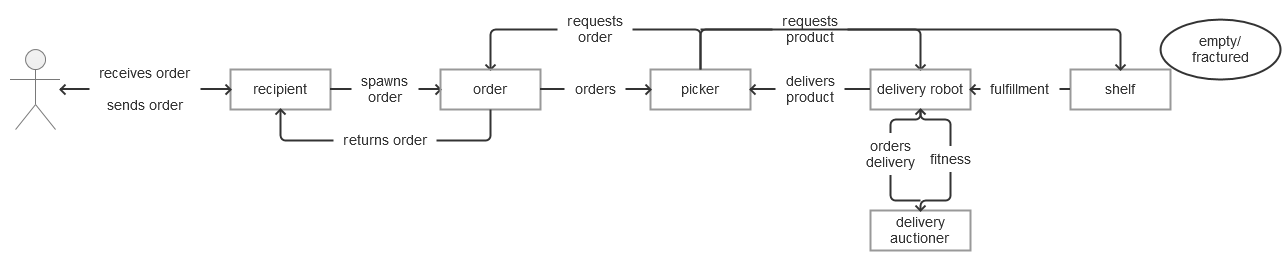
\includegraphics[width=10cm]{architecture_old.png}
 %\caption{}
\end{figure}

\bigskip

\begin{figure}
 \center
 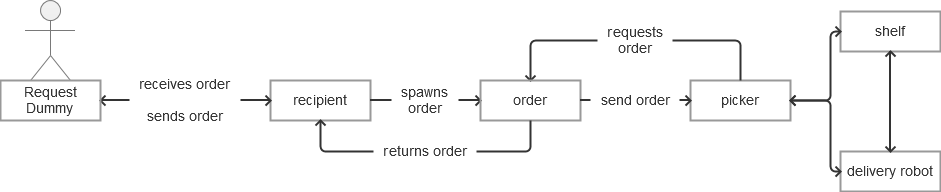
\includegraphics[width=10cm]{architecture_new.png}
 %\caption{}
\end{figure}

\end{frame}



\begin{frame}[fragile]
\frametitle{Communication}
\framesubtitle{}

\begin{columns}[t,onlytextwidth]
\column{.3\textwidth}

\begin{figure}
 \center
 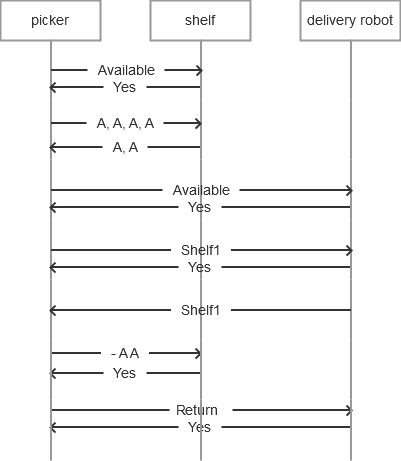
\includegraphics[width=4cm]{communication.png}
 %\caption{}
\end{figure}

\column{.6\textwidth}
Good:
\footnotesize
\begin{lstlisting}[language=Java]
inform = myAgent.receive(MessageTemplate.MatchPerformative(ACLMessage.INFORM));
					
if (confirm != null) {
...\end{lstlisting}
\normalsize
\bigskip
Bad:
\footnotesize
\begin{lstlisting}[language=Java]
informing_free = new ReceiverBehaviour(this, timeout, MessageTemplate.MatchPerformative(ACLMessage.INFORM));

if (informing_free.done()) {
...
\end{lstlisting}

\end{columns}

\end{frame}


\begin{frame}[fragile]
\frametitle{Challenges}
\framesubtitle{Best of in chronological order}

Commits:
\begin{itemize}
\item request dummy added
\item Broadcast via DFService 'giveOrder' implemented
\item picker refactored
\item overflow resolved by removing receiverBehaviour
\item changed String[] to List$<$String$>$ (Order)
\item Almost Complete
\end{itemize}

\end{frame}

\begin{frame}[fragile]
\frametitle{Demo + Code}
\framesubtitle{}

\begin{itemize}
\item Spawn warehouse
	\begin{itemize}
	\item Spawn all other agents
	\item TakeDown()
	\end{itemize}
\item RequestDummy generates and spawns order
\item Picker $\leftrightarrow$ order\\
Lookup, request, acknowledge
\item Picker $\leftrightarrow$ shelves\\
Lookup, request products, answer
\item Picker decide which product need to be brought from which shelf
\item Picker $\leftrightarrow$  delivery robot\\
Lookup, availability, request delivery
\end{itemize}


\end{frame}


\begin{frame}[fragile]
\frametitle{\textbf{\textbackslash \textbackslash TODO}}
\framesubtitle{}

\begin{itemize}
\item Delivery robot $\rightarrow$ picker\\
Shelf is available
\item Picker $\leftrightarrow$ shelf\\
Decrease content, OK
\item Picker $\rightarrow$ delivery robot\\
Deposit Shelf
\item Picker $\rightarrow$ request dummy\\
OK, order.TakeDown()
\end{itemize}

\end{frame}



\begin{frame}[fragile]
\frametitle{Testing}
\framesubtitle{}

\begin{itemize}
\item Scale orders
\item Scale warehouse
\item What if a shelf is empty?
\item All agents should check whether their successor is still working (randomly kill agents)
\item Improve shelf choice
\item Improve delivery robot choice
\item Think about shelves on robots
\item Add visualisation
\item Add position to shelves and delivery robots
\end{itemize}

\end{frame}

%COPY AND PASTE FROM HERE

%\begin{enumerate}
% \item 
%\end{enumerate}

%\hyperref[link]{text}

%\begin[Language=Python]{lstlisting}
%#PYTHON CODE HERE
%\end{lstlisting}

%\lstinputlisting[Language=Python]{ }

%\begin{figure}
% \center
% \includegraphics[width= cm]{ }
% \caption{}
%\end{figure}

%BIBLIOGRPAHY?
%\bibliographystyle{ieee}%amsalpha
%\bibliography{ }

\end{document}
